\documentclass[12pt,a4paper]{article}

% Packages
\usepackage[utf8]{inputenc}
\usepackage[T1]{fontenc}
\usepackage{lmodern}
\usepackage{geometry}
\usepackage{xcolor}
\usepackage{fancyhdr}
\usepackage{listings}
\usepackage{amsmath,amssymb}
\usepackage{graphicx}
\usepackage{booktabs}
\usepackage{tabularx}
\usepackage{parskip}
\usepackage{eso-pic}
\usepackage{hyperref}
\usepackage{float}
\usepackage{caption}
\usepackage{array}

% Page Geometry
\geometry{left=2.5cm, right=2.5cm, top=2.8cm, bottom=2.8cm}

% Colour Palette
\definecolor{primaryblue}{RGB}{0,51,102}
\definecolor{accentblue}{RGB}{0,102,153}
\definecolor{codebg}{RGB}{248,248,248}
\definecolor{codeframe}{RGB}{200,200,200}
\definecolor{darkgreen}{RGB}{0,120,60}
\definecolor{darkred}{RGB}{160,30,30}

% Custom Box Environments
\newenvironment{foplbox}%
  {\vspace{6pt}\par\noindent{\color{accentblue}\hrule height 1pt}\vspace{4pt}\noindent\ignorespaces}%
  {\par\nopagebreak\noindent{\color{accentblue}\hrule height 1pt}\vspace{8pt}}

\newenvironment{tracebox}%
  {\vspace{6pt}\par\noindent{\color{darkgreen}\hrule height 0.8pt}\vspace{2pt}%
   \begin{quote}\small\ignorespaces}%
  {\end{quote}\nopagebreak\noindent{\color{darkgreen}\hrule height 0.8pt}\vspace{6pt}}

% Listings Style: Prolog
\lstdefinestyle{prolog}{%
  language=Prolog,
  basicstyle=\ttfamily\small,
  keywordstyle=\color{primaryblue}\bfseries,
  commentstyle=\color{gray}\itshape,
  stringstyle=\color{darkred},
  numberstyle=\tiny\color{gray},
  numbers=left, numbersep=6pt,
  frame=none,
  breaklines=true, showstringspaces=false,
  tabsize=2, captionpos=b,
  xleftmargin=18pt,
  aboveskip=10pt, belowskip=6pt
}

% Listings Style: Python
\lstdefinestyle{python}{%
  language=Python,
  basicstyle=\ttfamily\small,
  keywordstyle=\color{primaryblue}\bfseries,
  commentstyle=\color{gray}\itshape,
  stringstyle=\color{darkred},
  numberstyle=\tiny\color{gray},
  numbers=left, numbersep=6pt,
  frame=none,
  breaklines=true, showstringspaces=false,
  tabsize=2, captionpos=b,
  morekeywords={True,False,None},
  xleftmargin=18pt,
  aboveskip=10pt, belowskip=6pt
}

% Listings Style: Output
\lstdefinestyle{output}{%
  basicstyle=\ttfamily\small,
  frame=none,
  breaklines=true, captionpos=b,
  xleftmargin=18pt,
  aboveskip=8pt, belowskip=4pt
}

% Section Formatting
\makeatletter
\renewcommand{\section}{\@startsection{section}{1}{\z@}%
  {-3.0ex \@plus -1ex \@minus -.2ex}%
  {1.5ex \@plus.2ex}%
  {\normalfont\Large\bfseries\color{primaryblue}}}
\renewcommand{\subsection}{\@startsection{subsection}{2}{\z@}%
  {-2.5ex\@plus -1ex \@minus -.2ex}%
  {1.0ex \@plus .2ex}%
  {\normalfont\large\bfseries\color{accentblue}}}
\renewcommand{\subsubsection}{\@startsection{subsubsection}{3}{\z@}%
  {-2.0ex\@plus -1ex \@minus -.2ex}%
  {0.8ex \@plus .2ex}%
  {\normalfont\normalsize\bfseries\color{accentblue!80!black}}}
\makeatother

% Header / Footer
\pagestyle{fancy}
\fancyhf{}
\fancyhead[L]{\small\textit{Lab Report --- Genetic Algorithms in AI}}
\fancyhead[R]{\small\textit{Nabina Thapa (080BCT047)}}
\fancyfoot[C]{\thepage}
\renewcommand{\headrulewidth}{0.4pt}
\renewcommand{\footrulewidth}{0.4pt}

% Hyperref Setup
\hypersetup{colorlinks=true, linkcolor=black, urlcolor=black}

\begin{document}

% COVER PAGE (bordered, plain style)
\thispagestyle{empty}
\AddToShipoutPictureBG*{%
  \AtPageLowerLeft{%
    \hspace{1.2cm}\raisebox{1.2cm}{%
      \color{black}\framebox[\dimexpr\paperwidth-2.4cm\relax]{%
        \rule{0pt}{\dimexpr\paperheight-2.4cm\relax}}%
    }%
  }%
}

\begin{center}

\vspace*{1.4cm}

\includegraphics[width=0.22\textwidth]{emblem.png}\\[0.6cm]

{\Large TRIBHUVAN UNIVERSITY}\\[0.35cm]
{\large INSTITUTE OF ENGINEERING}\\[0.15cm]
{\large PULCHOWK CAMPUS}\\[1.4cm]

{\bfseries\large A LAB REPORT\\
ON\\[0.2cm]
Genetic Algorithms in AI}

\vspace{2.2cm}

{\rule{0.3pt}{2.3cm}}\hspace{1.4cm}{\rule{0.3pt}{2.3cm}}\hspace{1.4cm}{\rule{0.3pt}{2.3cm}}

\vspace{2.6cm}

\end{center}

\noindent
\begin{minipage}[t]{0.47\textwidth}
\vspace{0pt}
\underline{\textbf{SUBMITTED BY:}}\\[0.4cm]
Name: Nabina Thapa\\[0.2cm]
Roll No.: 080BCT047\\[0.2cm]
Lab No.: 06
\end{minipage}\hfill
\begin{minipage}[t]{0.47\textwidth}
\vspace{0pt}
\begin{flushright}
\underline{\textbf{SUBMITTED TO:}}\\[0.4cm]
Department of Electronics\\[0.2cm]
and Computer Engineering
\end{flushright}
\end{minipage}

\vfill
\clearpage
\setcounter{page}{1}

% TABLE OF CONTENTS
\tableofcontents
\newpage

\section{Objectives}

\begin{enumerate}
  \item To understand how a genetic algorithm represents a local control policy as a chromosome.
  \item To model the painter robot using a lookup table based on its current square and local surroundings.
  \item To evolve a population of 50 chromosomes for 200 generations in a 20 by 40 empty room.
  \item To compare the evolved policy in an empty room with its behaviour in a furnished room containing 100 obstacle cells.
  \item To study the effects of selection, crossover, mutation, repeated trials, and final-population visualisation.
\end{enumerate}

\section{Theory}

A genetic algorithm searches for good solutions by maintaining a population of candidate chromosomes.  Each chromosome is evaluated with a fitness function, and better candidates are more likely to contribute genes to the next generation.  Crossover combines parent chromosomes, while mutation preserves variation by changing selected genes.

\subsection{Chromosome and State Representation}

The painter robot does not store a complete map of the room.  Instead, its action is selected from a table indexed by the local state
\[
  [c,f,l,r],
\]
where $c$ records whether the current square is painted, and $f$, $l$, and $r$ describe the forward, left, and right cells.  The current square has two possible values and each neighbouring cell has three possible values, giving
\[
  2 \times 3 \times 3 \times 3 = 54
\]
possible states.  Therefore, one chromosome contains 54 genes.  Each gene stores one of four actions: no turn, turn left, turn right, or choose a random left/right turn.

\subsection{Fitness}

The fitness of a chromosome is the fraction of all reachable empty cells that are painted before the safety horizon is reached:
\[
  F = \frac{\text{number of painted empty cells}}
           {\text{number of paintable cells}}.
\]
The experiment uses three starting states while evolving a chromosome and eight starting states for validation.  Averaging over several starts reduces the chance that a policy is selected only because of one convenient initial position.

\subsection{Obstacle Layout}

The furnished-room experiment uses the same 20 by 40 room with three rectangular furniture blocks.  The blocks occupy exactly 100 cells, leaving 700 paintable cells.  A chromosome evolved in the empty room is first transferred without retraining, and a second population is then evolved directly in the furnished room.

\section{Methodology}

The experiment was implemented in Python 3.  The state table is generated from the Cartesian product of the four local observations, and the robot simulator returns both the coverage fraction and the complete trajectory.  A fixed seed of 40731 was used so that the saved figures and summary values can be reproduced.

The independent implementation uses rank-weighted parent sampling, two-point crossover, three elite chromosomes, and a mutation rate of 0.0025.  Whenever a gene mutates, it is replaced by a different action.  Each population contains 50 chromosomes and is evolved for 200 generations.

\begin{center}
\begin{tabular}{ll}
\toprule
\textbf{Parameter} & \textbf{Value} \\
\midrule
Population size & 50 chromosomes \\
Chromosome length & 54 genes \\
Generations & 200 \\
Training starts & 3 per chromosome \\
Validation starts & 8 \\
Selection & Rank-weighted sampling with 3 elites \\
Crossover & Two-point crossover \\
Mutation probability & 0.0025 per gene \\
\bottomrule
\end{tabular}
\end{center}

\begin{figure}[H]
\centering
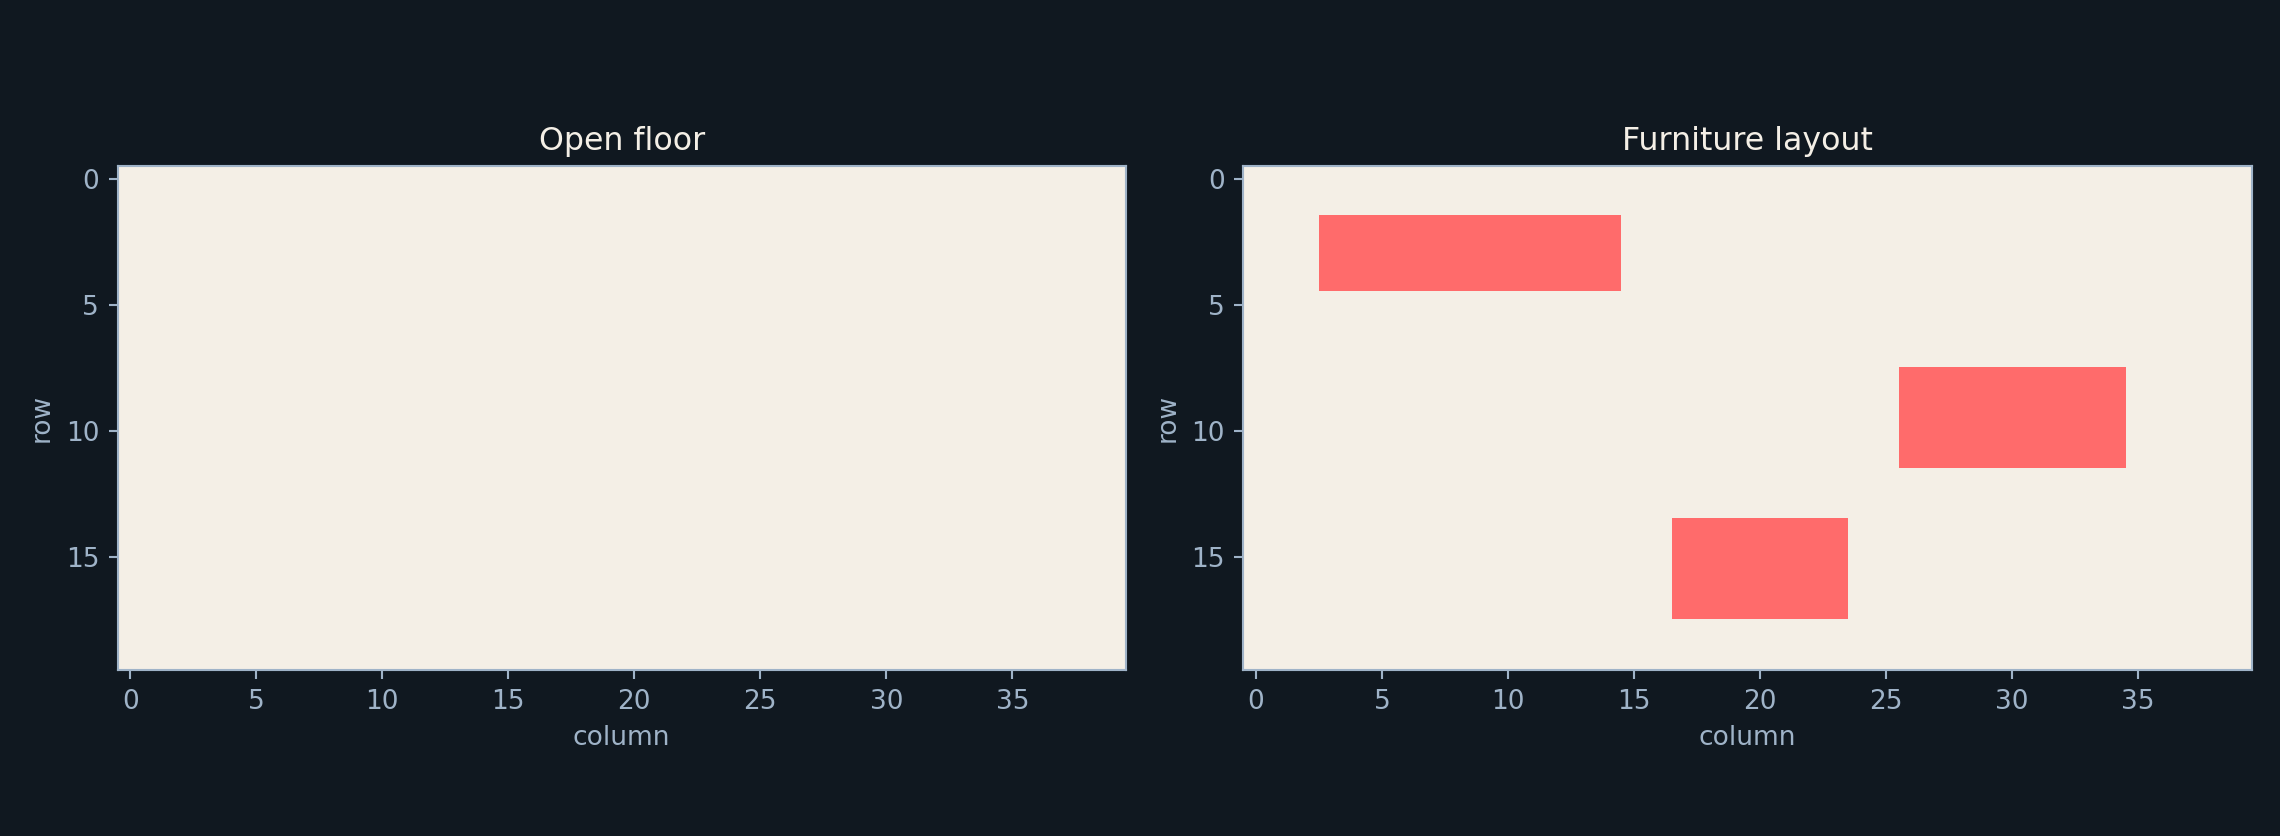
\includegraphics[width=0.82\textwidth]{outputs/room_layouts.png}
\caption{Empty room and the 100-cell furnished-room layout.}
\end{figure}

\section{Implementation}

\subsection{Simulation and Genetic Operators}

The file \texttt{code/redone\_painter\_ga.py} contains the simulator, genetic operators, validation routines, and plotting functions.  The robot paints its current cell, reads the four local observations, applies the action stored at the corresponding gene, and attempts to move forward.  Invalid moves are counted in the trajectory but do not paint a new cell.

The main command used to generate the experiment is:

\begin{tracebox}
\begin{verbatim}
python code/redone_painter_ga.py --output outputs
\end{verbatim}
\end{tracebox}

The output directory contains the room layouts, generation curves, final chromosome heat maps, trajectories, CSV fitness histories, and a JSON summary of the numerical results.

\subsection{Assignment 1 Strategy}

Before evolution, a simple hand-designed strategy for the empty room is a boustrophedon sweep.  The robot traverses one row, turns at the boundary, shifts by one row, and traverses the next row in the opposite direction.  This strategy reduces repeated long walks and gives a useful reference for judging the evolved local policy.

\subsection{Assignment 3 Innovations}

Two local innovations that can produce a sudden increase in fitness are:
\begin{enumerate}
  \item A forward-block rule that turns toward an open side when the forward cell is a wall or furniture.
  \item A painted-neighbour rule that treats an already painted strip as a boundary and directs the robot toward the adjacent unpainted strip.
\end{enumerate}
Both innovations convert local observations into approximate memory of the route without adding an explicit global map.

\section{Results}

\subsection{Empty Room}

The best empty-room chromosome reached complete coverage for one validation start and achieved a mean coverage of 97.77\% over eight validation starts.  The weakest validation start covered 88.00\% of the 800 paintable cells.

\begin{table}[H]
\centering
\caption{Empty-room result summary}
\begin{tabular}{@{}lr@{}}
\toprule
\textbf{Measure} & \textbf{Result} \\
\midrule
Paintable cells & 800 \\
Mean coverage & 97.77\% \\
Best validation run & 100.00\% \\
Weakest validation run & 88.00\% \\
Mean steps & 2096.75 \\
\bottomrule
\end{tabular}
\end{table}

\begin{figure}[H]
\centering
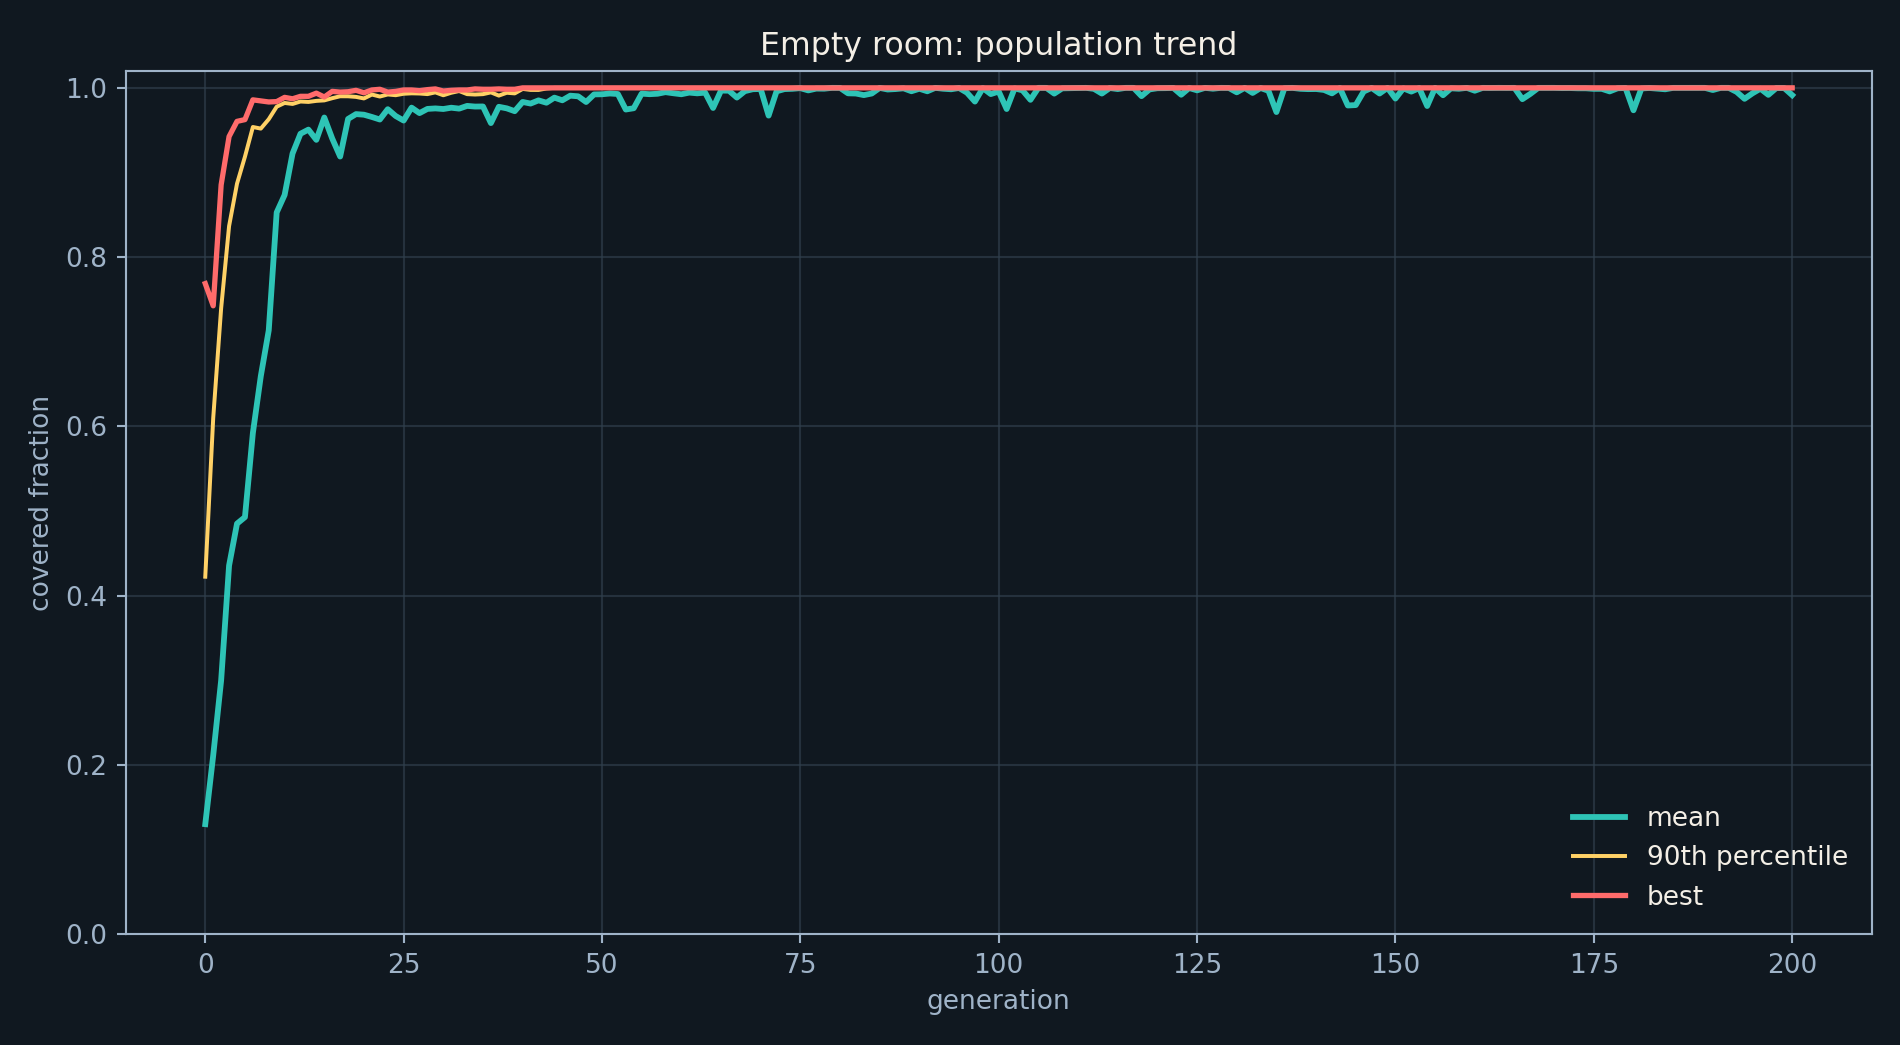
\includegraphics[width=0.88\textwidth]{outputs/empty_fitness.png}
\caption{Mean, 90th-percentile, and best fitness across empty-room generations.}
\end{figure}

\begin{figure}[H]
\centering
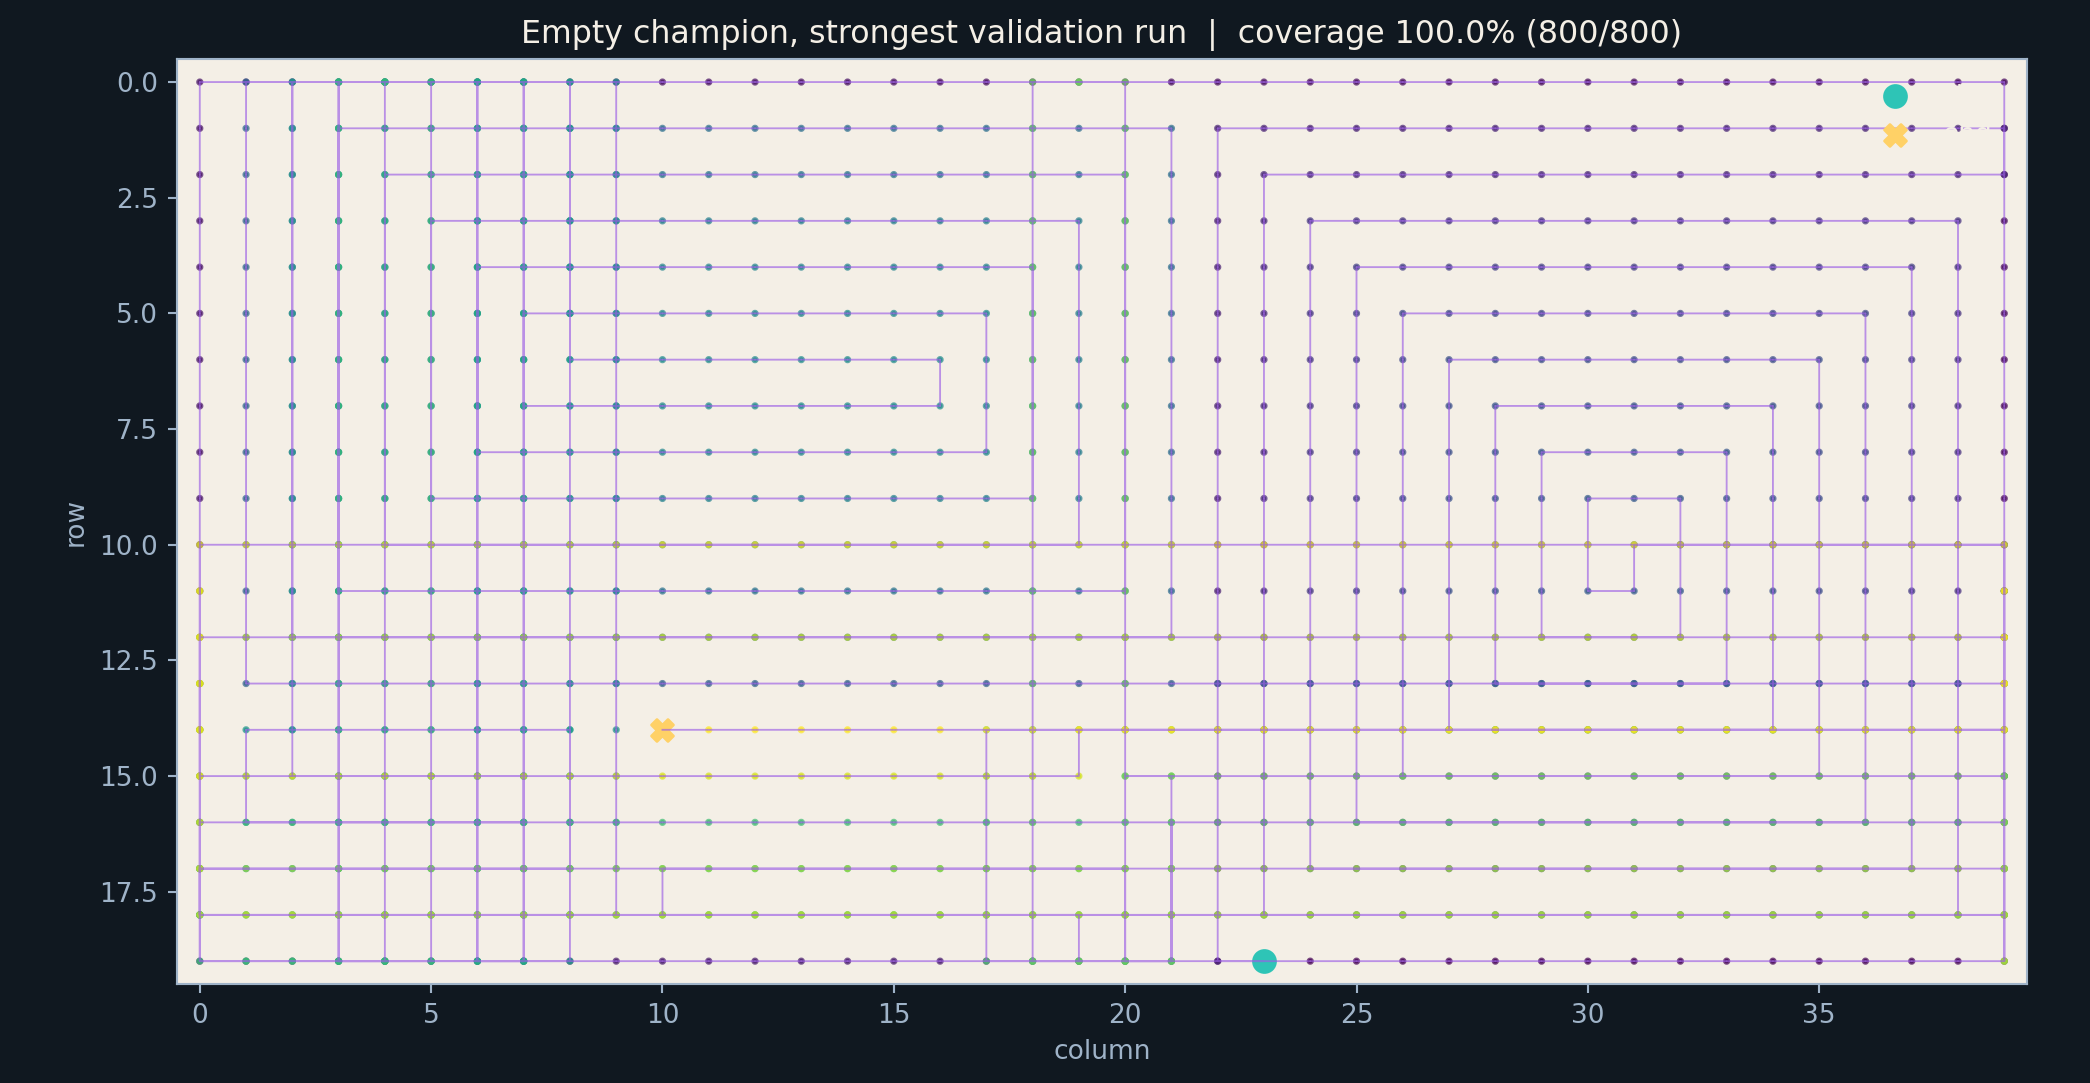
\includegraphics[width=0.88\textwidth]{outputs/empty_trajectory_best.png}
\caption{Trajectory of the strongest empty-room validation run.}
\end{figure}

\subsection{Final Population}

The final chromosome heat map shows the action selected for every state in all 50 chromosomes.  Repeated vertical bands indicate states where selection converged toward a common action, while irregular bands indicate states that remain sensitive to the route history.

\begin{figure}[H]
\centering
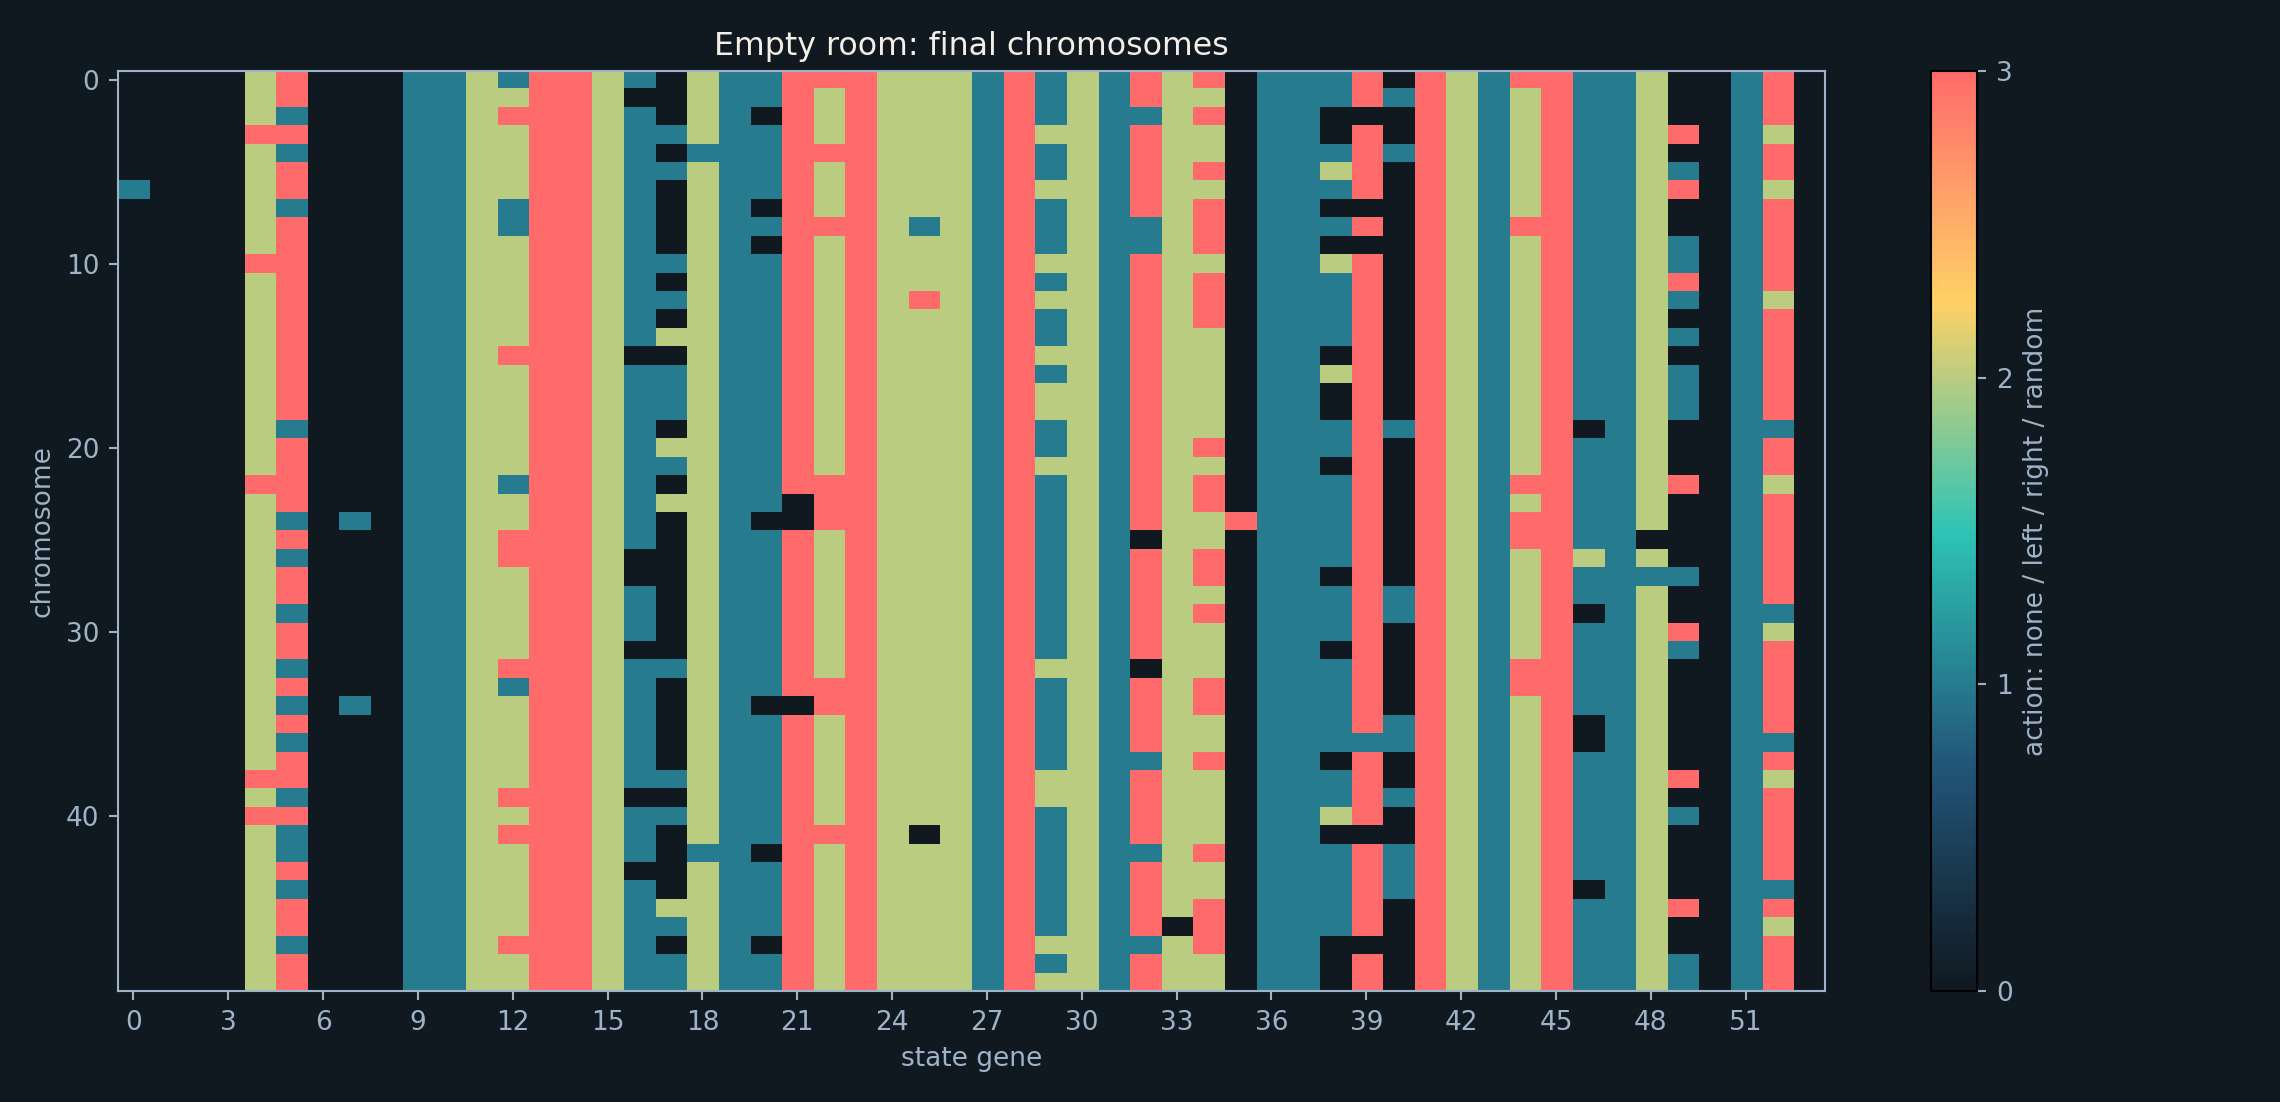
\includegraphics[width=0.90\textwidth]{outputs/empty_population.png}
\caption{Final population after evolution in the empty room.}
\end{figure}

\subsection{Assignment 4: Furniture Transfer}

The empty-room champion was tested in the furnished room without retraining.  It achieved 96.84\% mean coverage over 700 paintable cells.  A new population evolved directly in the furnished room achieved 97.36\% mean coverage.

\begin{table}[H]
\centering
\caption{Transfer and furnished-room comparison}
\begin{tabular}{@{}lrrrr@{}}
\toprule
\textbf{Test} & \textbf{Mean} & \textbf{Best} & \textbf{Weakest} & \textbf{Cells} \\
\midrule
Empty champion transferred & 96.84\% & 100.00\% & 91.71\% & 700 \\
Furnished room evolved directly & 97.36\% & 100.00\% & 84.29\% & 700 \\
\bottomrule
\end{tabular}
\end{table}

\begin{figure}[H]
\centering
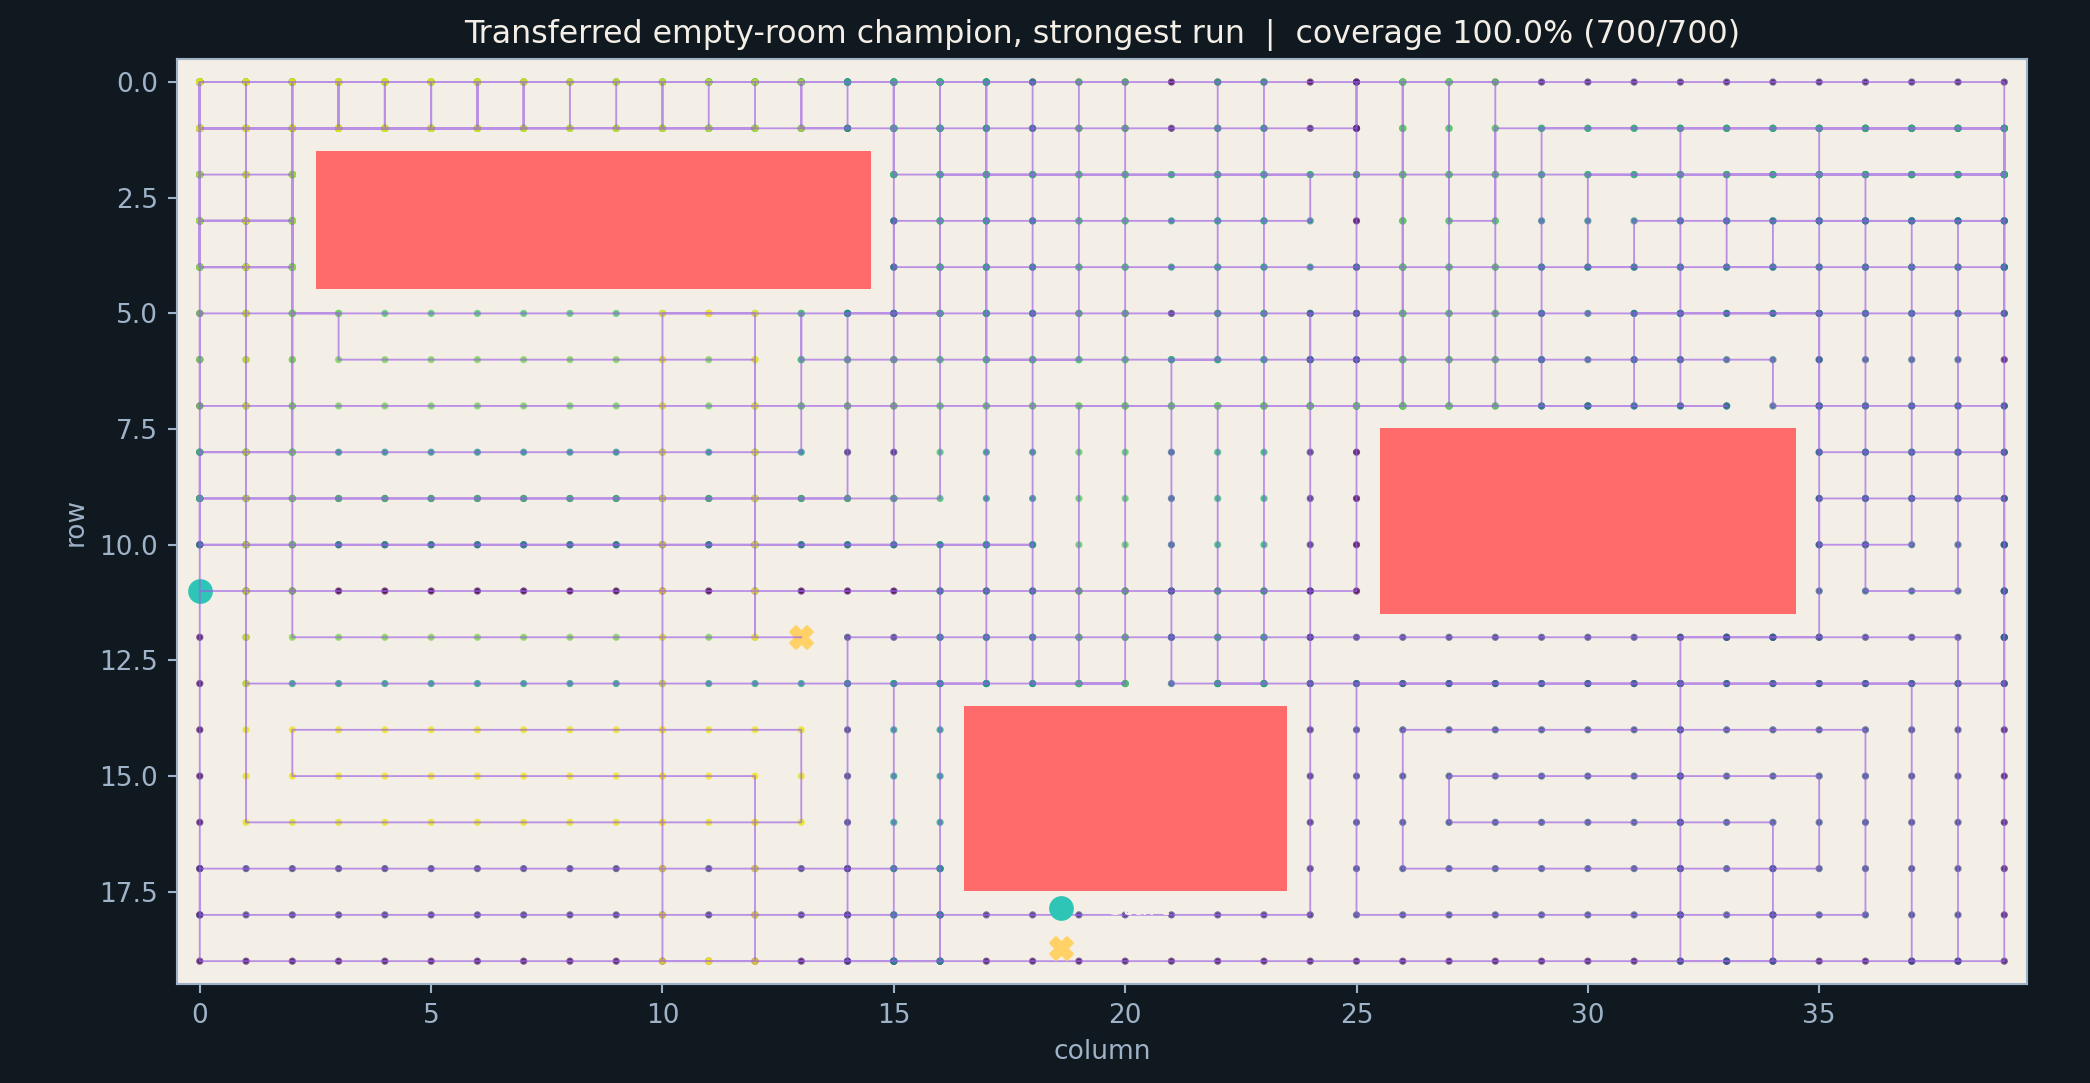
\includegraphics[width=0.44\textwidth]{outputs/transfer_best.png}\hspace{0.04\textwidth}
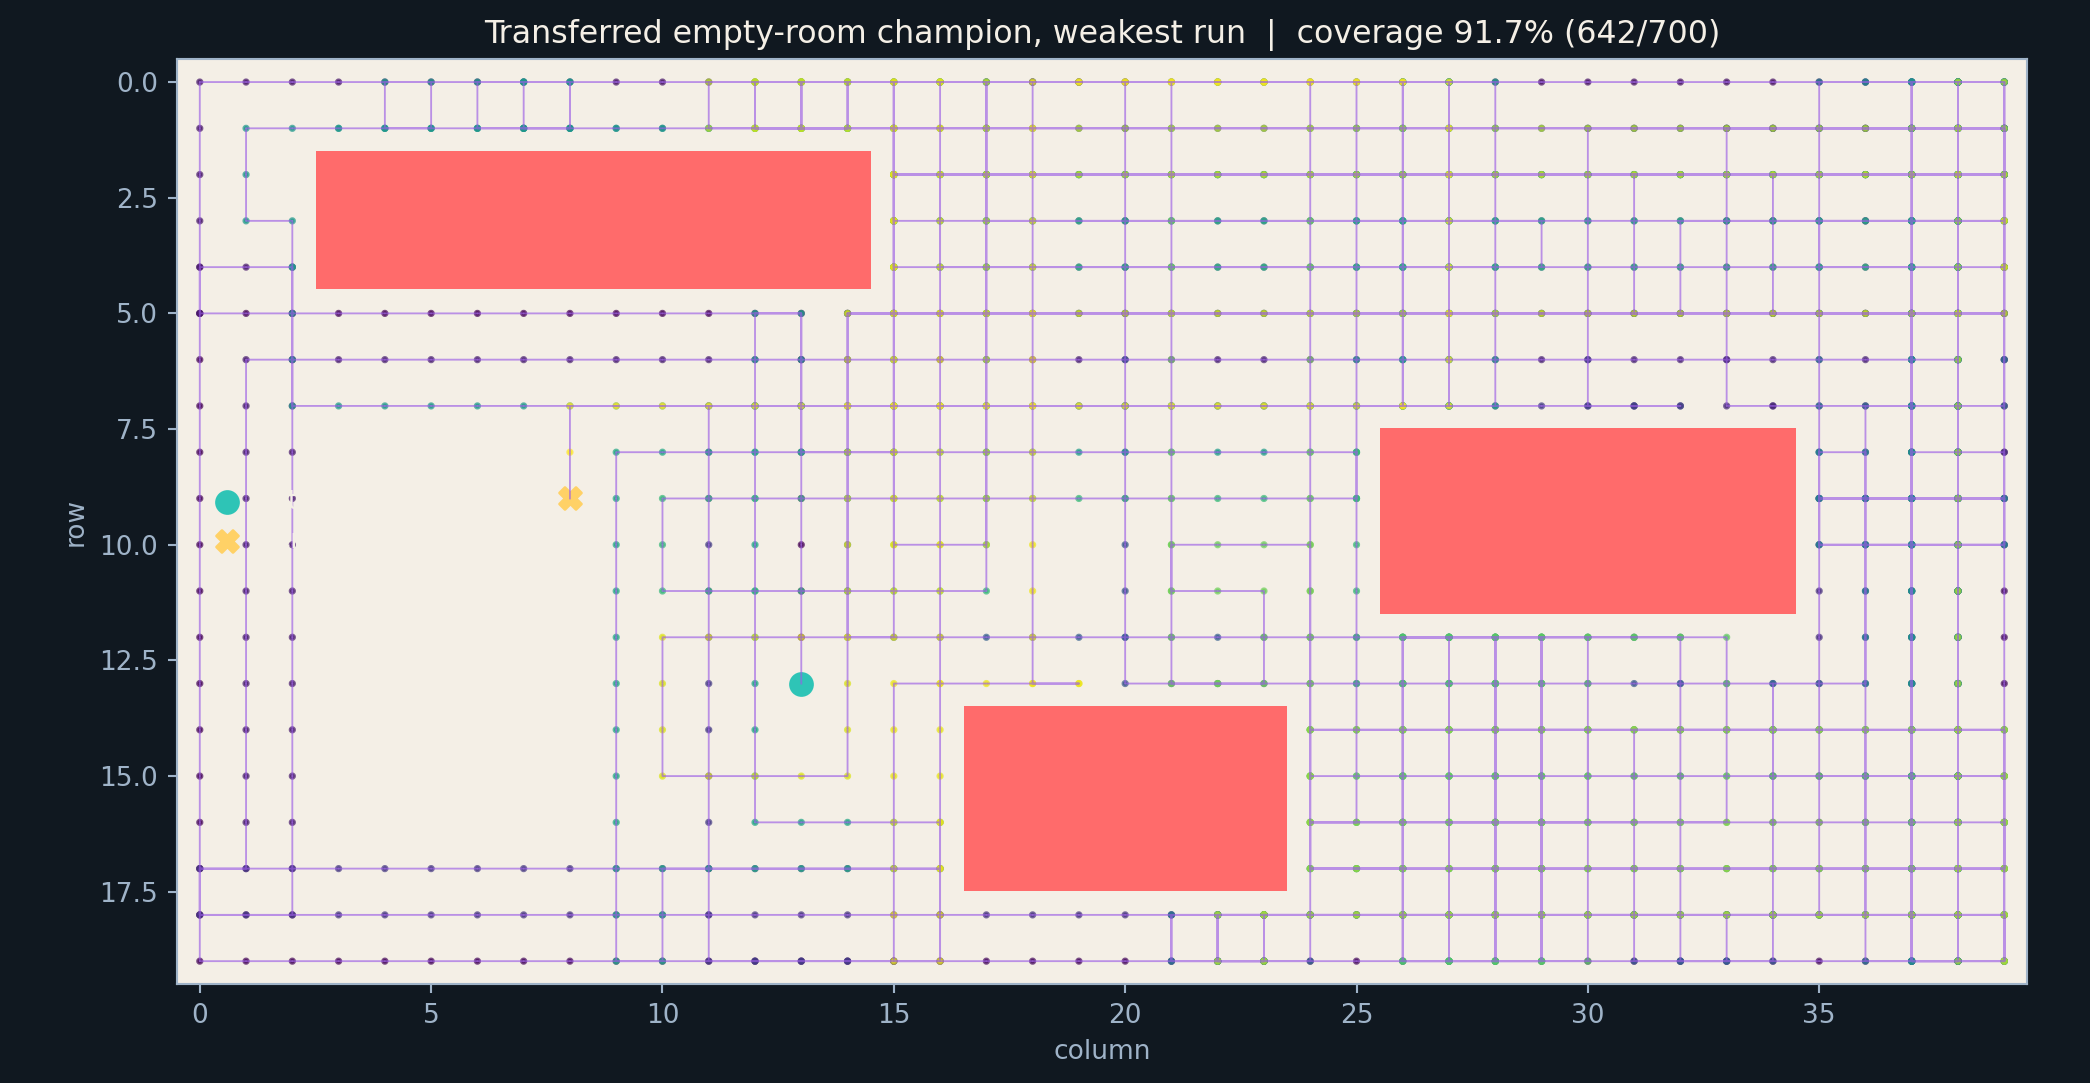
\includegraphics[width=0.44\textwidth]{outputs/transfer_weakest.png}
\caption{Strongest and weakest transfer trajectories in the furnished room.}
\end{figure}

\begin{figure}[H]
\centering
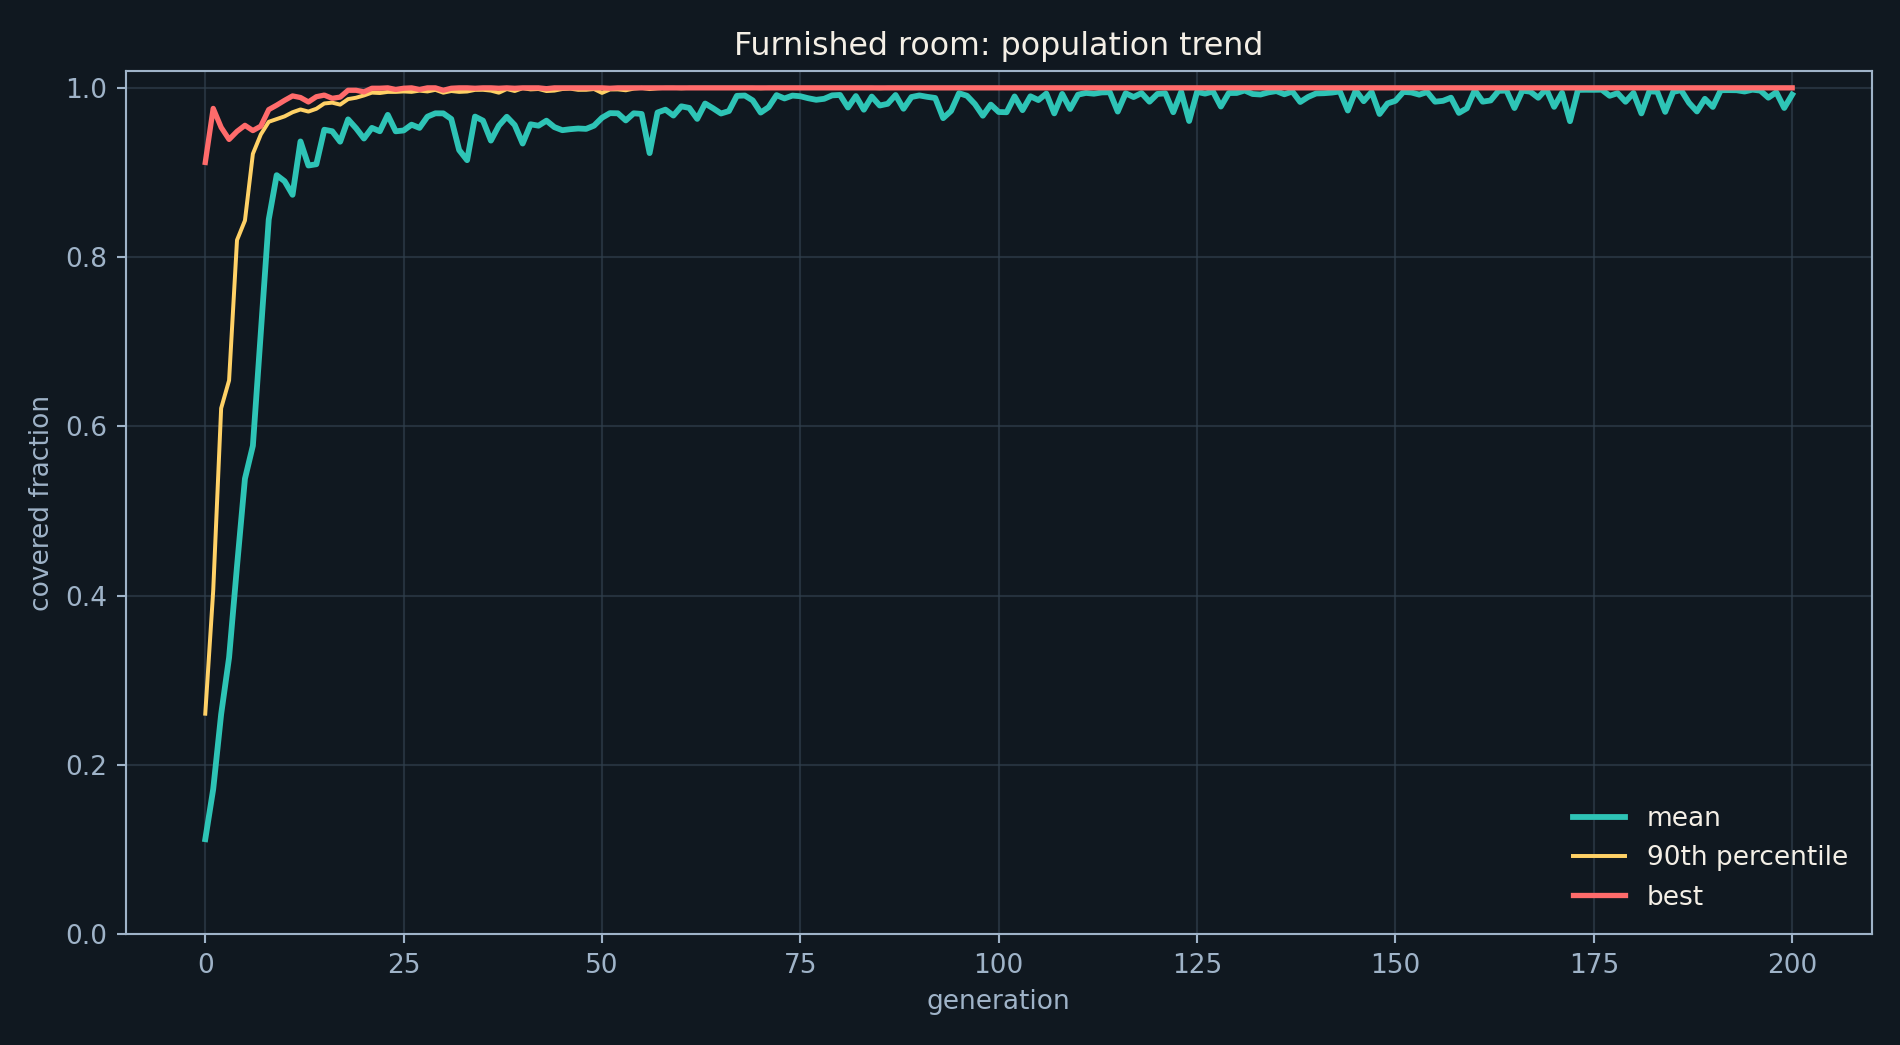
\includegraphics[width=0.88\textwidth]{outputs/furnished_fitness.png}
\caption{Fitness history during evolution in the furnished room.}
\end{figure}

\begin{figure}[H]
\centering
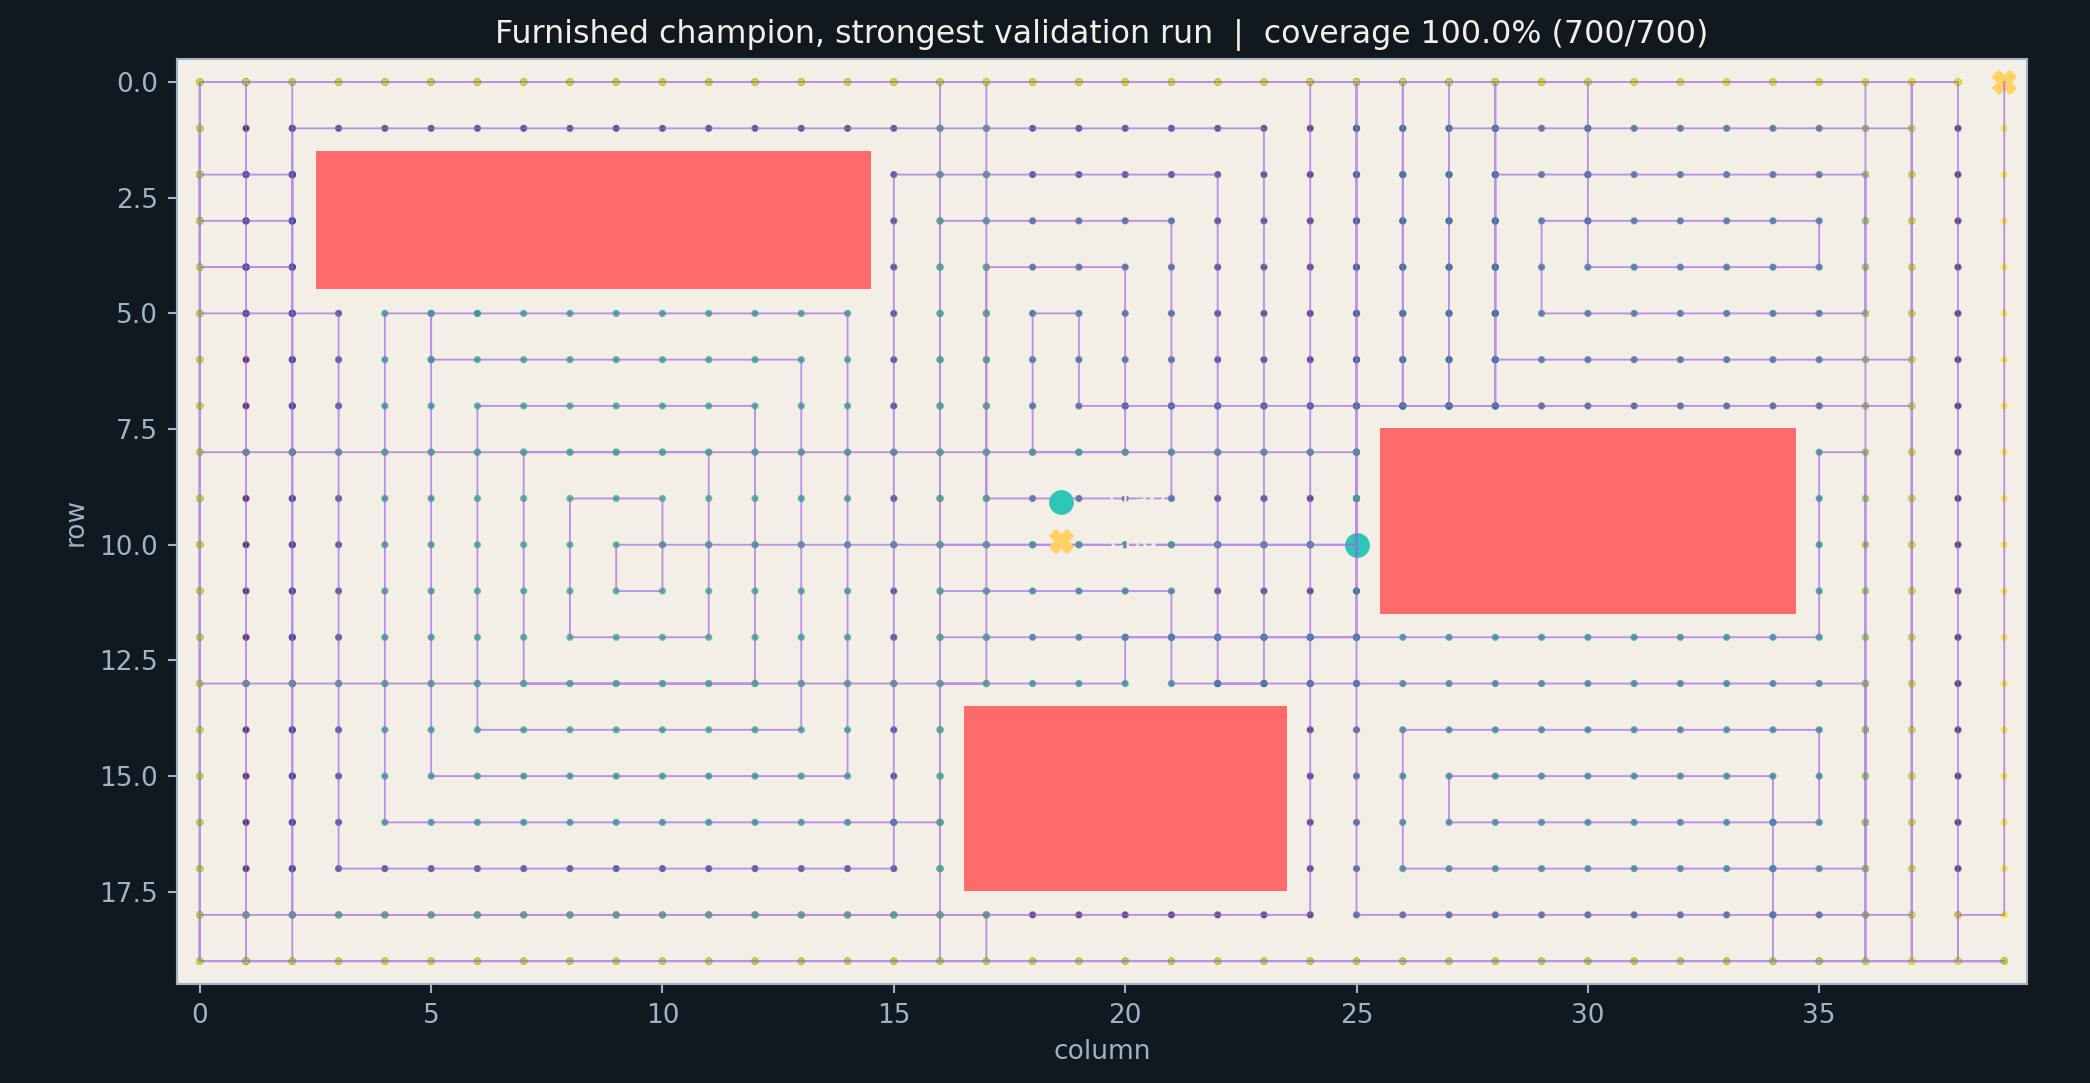
\includegraphics[width=0.88\textwidth]{outputs/furnished_trajectory_best.png}
\caption{Strongest validation trajectory for the furnished-room champion.}
\end{figure}

\begin{figure}[H]
\centering
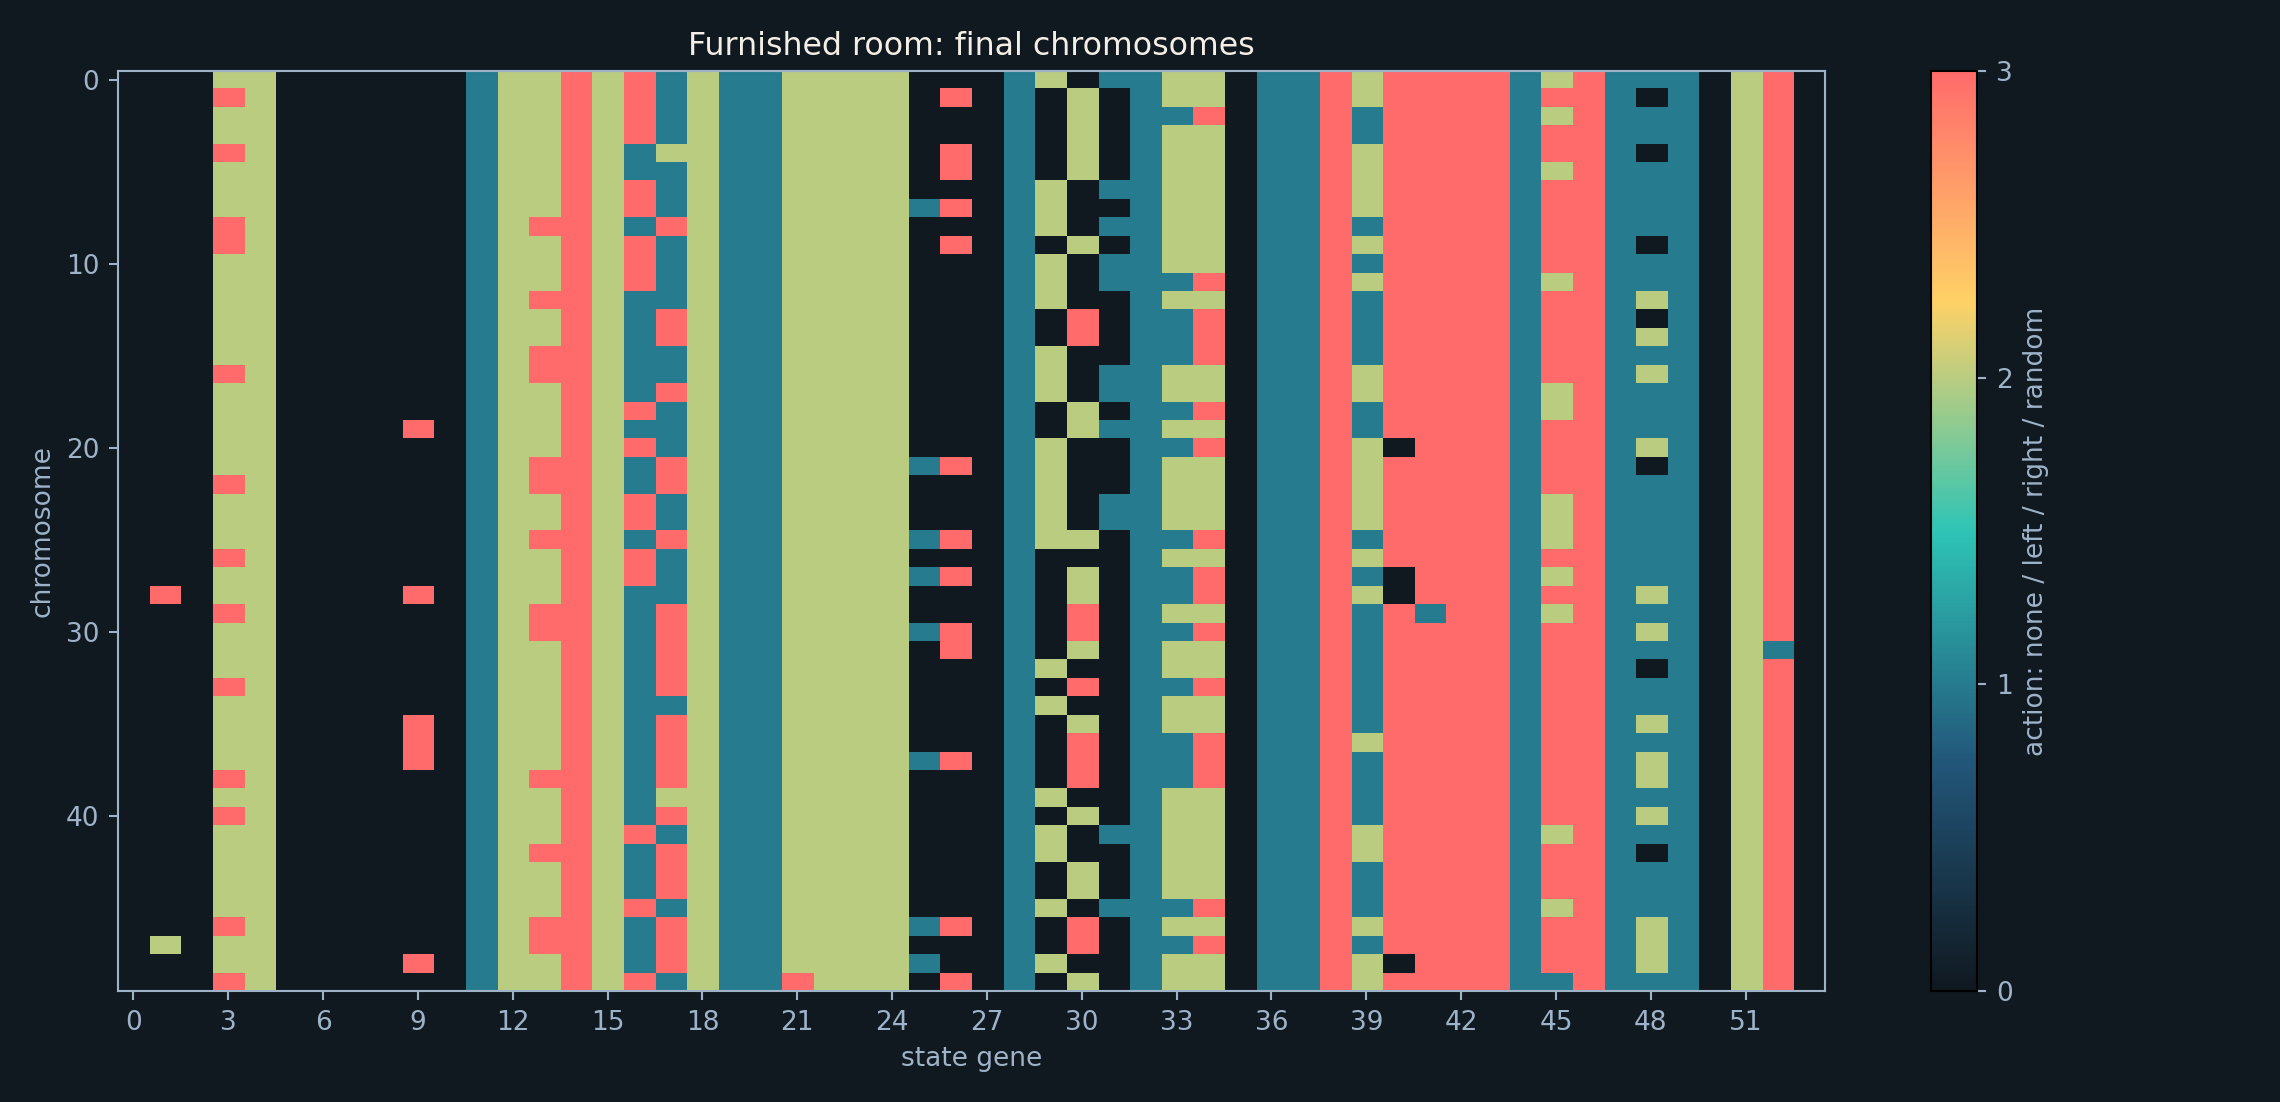
\includegraphics[width=0.90\textwidth]{outputs/furnished_population.png}
\caption{Final chromosome population after furnished-room evolution.}
\end{figure}

\section{Discussion}

The fitness curves rise rapidly during the first generations and then stabilise near complete coverage.  The best curve reaches a high value earlier than the mean curve because one successful local rule combination can appear before crossover spreads it through the rest of the population.

The empty-room chromosome transfers well to the furnished layout because several of its actions respond to local boundaries.  However, furniture changes the meaning of a useful turn: a rule that is helpful at an outside wall may cause a detour near a rectangular obstacle.  This explains why the transferred champion has a lower mean than its empty-room result and why the directly evolved furnished-room population is more obstacle-specific.

The results also show that the highest single validation score is not enough to describe a policy.  Both evolved champions achieved 100.00\% on one starting state, but their weakest validation runs were lower.  Repeated starts therefore provide a more reliable measure of general behaviour.

\section{Conclusion}

This lab demonstrated how a genetic algorithm can evolve a useful painter-robot policy from local observations.  A chromosome of only 54 action genes was evaluated, selected, recombined, and mutated over 200 generations.  In the alternate run, the empty-room champion averaged 97.77\% coverage, transferred to the furnished layout with 96.84\% coverage, and direct furnished-room evolution averaged 97.36\%.

The experiment confirms that genetic algorithms can discover compact control rules without explicitly programming a global route.  At the same time, the furniture experiment shows that performance depends on the environment and the starting state.  Selection, crossover, mutation, repeated validation, and trajectory plots together provide a practical way to analyse the quality and limitations of the evolved policy.

\end{document}
